\fancychapter{A Rapport Computational Model}
\label{chap:rapportModel}

Inspired by current literature on rapport~\cite{Buschmeier2011, Spencer-Oatey2005, Zhao2014, Papangelis2014} and social agents~\cite{Zwiers2011, Reidsma2011, Riek2009, Niewiadomski2009, Andrist2014, Andrist2015, Cassell2007, Wang2009, Schroder2010, Buschmeier2011, Tullio2015}, we selected the most prominent features that allows researchers to design agents (either virtual or robotic) capable of building rapport and establish closer relationships more efficiently with humans. For example, take into account any particular information regarding either the user or the task to tailor the interaction strategies and be more effective on managing rapport with people (Section~\ref{sec:ComputationalModelsOfRapport}) and take into account that nowadays, researchers have been building hybrid systems that can bring forth the advantages of rule-based systems and data-driven systems. Therefore, it is crucial that the rapport model follows its fundamentals concepts (Chapter~\ref{chap:rapport}), follows the ideas proposed by Zhao, Papangelis and Cassel~\cite{Zhao2014, Papangelis2014} (Section~\ref{sec:ComputationalModelsOfRapport}), and that provides the flexibility to design behavioural models that can be refined independently from one another either through rule-based designs, or through data-driven designs that are growing in the research community.

For this purpose, the built rapport model has the following goals:

\begin{itemize}
    \item Build rapport following its three levels: positivity, mutual attention and coordination as rapport is more effective when they are considered simultaneously during interactions~\cite{Buschmeier2011, Spencer-Oatey2005, Zhao2014, Papangelis2014};
    \item Support dynamic interruption and replacement of actions that is vital to design agents capable of adapting its actions to the external world that is continuously changing~\cite{Reidsma2011, Visser2014, Kopp2007, Zwiers2011}. For example, stop speaking whenever the agent perceives that it another person wishes to take its turn;
    \item Permit concurrent execution of actions, that is, model agents capable of, for example, mimic facial expressions while nodding its head to show signs of attentiveness;
    \item Be sufficiently generic and customisable to tailor the agents to different embodiments and/or \ac{HRI} scenarios.
\end{itemize}

\section{Overview}

The rapport model takes into account the goal tree depicted in Figure~\ref{table:rapportModel}, for example, in order to enhance mutual attention, the agent should produce listener behaviour (backchannel) and establish gaze contact with the person. As detailed previously in Chapter~\ref{chap:rapport}, there may be other goals such as maintain of even destroy rapport that impacts the goal tree, however, this thesis focus solely on strategies for building rapport.

\begin{figure}[H]
    \centering
    %\begin{framed}
        \scalebox{0.7}{
            \begin{forest}
                [\textbf{Build Rapport}
                    [Stimulate Positivity 
                        [Self-disclosure][Motivate][Humor]]
                    [Stimulate Mutual Attention
                        [Mutual Gaze][Backchannel]]
                    [Stimulate Coordination
                        [Behavioural Mimicry
                            [Facial Expressions][Head Gestures]]
                        [Adhere To Social Norms]
                        [Backchannel]]
                ]               
            \end{forest}
        }
    %\end{framed}
    \caption{Goal tree of the rapport model. The nodes are goals and the leafs are actions.}
    \label{table:rapportModel}
\end{figure}

In order to make the agent more effective, it should adapt its interaction strategies to both the partner and the surrounding environment. For example, it would be a mistake the agent to behave differently than what the society expect of it. In addition, the agent should also be able to adapt at any time to changes of the environment, for example, it should be able to stop speaking at any time to give the turn to others to speak, possibly apologising for taking the time for doing it~\cite{Buschmeier2011}. For this purpose, the dyadic state of the interaction should be stored and used by the agent.

Following Figure~\ref{fig:rapportModel}, the rapport model has the following components:
\begin{itemize}
    \item \textbf{Dyadic State}: contains information regarding the interactional partner and the environment;
    \item \textbf{Perceptions}: perceptual information;
    \item \textbf{Rapport Effectors}: components that generate signs of rapport by proposing actions to the \textit{Rapport Controller} given the dyadic state of the interaction;
    \item \textbf{Rapport Controller}: manages the proposed actions sent by the rapport \textit{Effectors}. Conflicts may arise causing interruption and/or replacement of actions.
\end{itemize}

\begin{figure}[H]
    \centering
    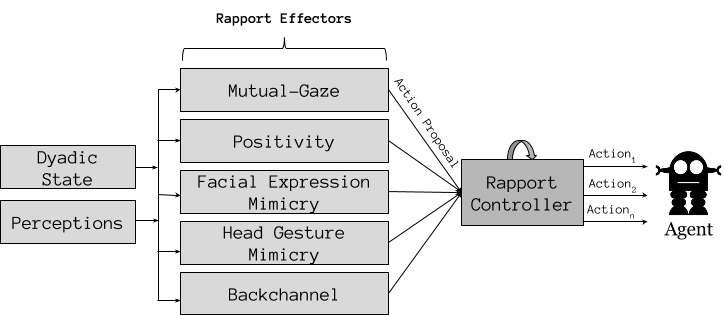
\includegraphics[width=0.9\textwidth]{images/RapportModel.png}
    \caption{Schematic representation of the rapport model.}
    \label{fig:rapportModel}
\end{figure}

The rapport \textit{Effectors} in Figure~\ref{fig:rapportModel} are independent allowing researchers to refine them separately. Additional \textit{Effectors} may be developed to complement/replace the existing ones. For example, at first, the backchannel component in Figure~\ref{fig:rapportModel} is a rule-based component that takes into account prosodic features (Section~\ref{sec:mutual_attentionModel}), however, in the future, it may be replaced by a data-driven model capable of detecting subtleties of the human behaviour more accurately.

\section{Rapport Controller}
\label{sec:rapportController}

The main responsibility of the \textit{Rapport Controller} is to manage the proposed actions sent by the different rapport strategies. Each action proposal is a quintuple $A= <G,P,E,I,T>$ containing:

\begin{itemize}
    \item \textbf{Group ($G$)}: part of agent's body that the action is attempting to manipulate. This gives more expressivity to the agent, as speaking (a \textit{Speech Group}) does not necessary interrupts a facial expression (a \textit{Face Group});
    \item \textbf{Priority ($P$ where $P \in \mathbb{N}_0$)}: relative importance of the action proposal in relation to others; 
    \item \textbf{Execution description ($E$)}: how the agent will execute the action;
    \item \textbf{Interruption description ($I$)}: how the action should be interrupted by the agent;
    \item \textbf{Timeout ($T$ where $T \in \mathbb{N}$)}: maximum duration of the action.
\end{itemize}

Concerning the management of action proposals, the controller periodically captures a snapshot of the agent's ongoing actions and pending action proposals received by the different \textit{Effectors}. Whenever a snapshot is captured or, when receiving a new action proposal, the controller analyses which actions should be interrupted (and replaced) using $I$. Following Figure~\ref{fig:no_conflicts}, as long as two action proposals have different groups ($S_G \neq A_G$), both will be executed using $S_E$ and $A_E$. However, following Figure~\ref{fig:conflict_interrupt}, in the case of a conflict ($A_{1_G}=A_{2_G}$), the action with the lowest priority is interrupted (orange area) and replaced by the newer action proposal. If the new action has lower priority than the current in execution, then it is ignored (Figure~\ref{fig:conflicting_not_interrupted}). Moreover, the action can be time limited, therefore, if the action takes longer than expected ($T$) it is interrupted, despite having higher priority.

\begin{figure}[H]
    \centering
    \begin{minipage}[b]{.4\textwidth}
        \centering
        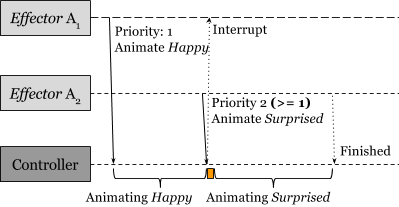
\includegraphics[width=\textwidth]{images/ConflictingAndInterrupt.png}
        \caption{Depiction of an incoming action proposal with the same \textit{Group} but with higher priority.}
        
        %The action with higher priority interrupts (orange area) and replaces the action in execution.
               
        \label{fig:conflict_interrupt}
    \end{minipage}
    \hspace{20mm}
%   \hfill
    \begin{minipage}[b]{.4\textwidth}
        \centering
        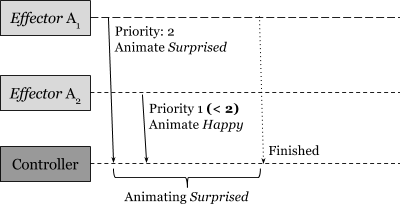
\includegraphics[width=\textwidth]{images/ConflictingNotInterrupted.png}
        \caption{Depiction of an incoming action proposal with the same \textit{Group} but with lower priority.}
        \label{fig:conflicting_not_interrupted}
    \end{minipage}
\end{figure}

%The action with lower priority is ignored as there is another action with the same \textit{Group} with higher priority is being executed.

\begin{figure}[H]
    \centering
    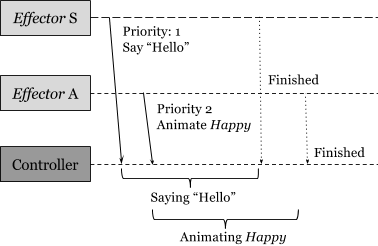
\includegraphics[width=0.4\textwidth]{images/NoConflicts.png}
    \caption{Depiction of an incoming action proposal with different \textit{Group}.}
    \label{fig:no_conflicts}
\end{figure}

%As the actions refer different \textit{Groups} there are not conflicting, and both will executed 

Lastly, the priority should be defined by the researcher. However, as rule of thumb, idle actions should have a lower priority than actions triggered by discrete states. For example, a surprise animation (as a reaction to something that just happened) should have higher priority than any idle animation.

\section{Stimulate Positivity}
\label{sub:model_positivity}

In pursuance of enhancing the first component of rapport, positivity, the Positivity \textit{Effector} takes into account the current state of the interaction to trigger, for example, contextual vocalisations to motivate or praise the interactional partner. For example, in tutoring scenarios it is important to motivate the students to achieve better results, and, more importantly, to praise them when accomplishing tough tasks. In addition, the agent should share a personal information to the person (self-disclosure), as the current literature suggests that it plays an important role in closing relationships between two strangers~\cite{Kang2011}. The interactional states and the corresponding sentences are specified by the researcher and should tailor to the dyadic state of the interaction as much as possible. For instance, in the case of the Portuguese language, which highly inflected on the gender, there have to be distinct sentences for each gender. To conclude, Table~\ref{table:positivity_rule_examples} depicts examples of interactional utterances that the researcher may specify for an agent during a game of Chess.

\begin{table}[H]
	\centering
	\begin{tabular}{|l|l|}
	\hline
	\textbf{Interactional State} & \textbf{Utterance} \\ \hline
	After Introduction & \specialcell{Did you know that I learnt the castling move yesterday where one moves\\ the king and the tower at the same time?} \\ \hline
	Player loses the queen & Don't fret, your king is still well guarded! \\ \hline
	Agent loses a bishop & Well... this could have gone better! \\ \hline
	Before the last round & These last matches were a warm-up, get ready! \\ \hline
	\end{tabular}
	\caption{Example utterances depending on the dyadic state of the interaction.}
	\label{table:positivity_rule_examples}
\end{table}

\section{Stimulate Mutual Attention}
\label{sec:mutual_attentionModel}

In order to enhance the second component of rapport, mutual attention, the model focuses on mutual gaze and listener behaviour strategies.

The Mutual-Gaze \textit{Effector} bases on the work developed by Andrist et. al.,~\cite{Andrist2015} described in Section~\ref{sub:sec:gaze}. In short, it swaps between establishing eye contact with the participant and looking at the game during pre-determined periods of time according to the following conditions: current phase of the scenario (in-task or between-tasks) and the user's personality (introverted or extroverted). By default, the lengths are the ones specified in Table~\ref{table:gazetimes} in Section~\ref{sub:sec:gaze}, however, the researcher may change these values for his specific needs (Table~\ref{table:mutualGazeParameters}). In addition, the researcher has to specify where the gaze targets on both phases (in-task and between-tasks).

%

\begin{table}[H]
	\centering
	\begin{tabular}{|l|l|l|l|c|}
	\hline
	\multicolumn{3}{|c|}{\textbf{Parameter}} & \multicolumn{1}{c|}{\textbf{Description}} & \multicolumn{1}{c|}{\textbf{Range}} \\ \hline
	\multicolumn{3}{|l|}{In-task Gaze Priority} & Gaze priority during the in-task phase & $\mathbb{N}_0$ \\ \hline
	\multicolumn{3}{|l|}{Between-tasks Gaze Priority} & Gaze priority during the between-tasks phase & $\mathbb{N}_0$ \\ \hline
	\multirow{4}{*}{Extrovert} & \multirow{2}{*}{In-task} & Face & Gaze duration & $\mathbb{N}$ \\ \cline{3-5} 
	 &  & Task & Gaze duration & $\mathbb{N}$ \\ \cline{2-5} 
	 & \multirow{2}{*}{Between-tasks} & Face & Gaze duration & $\mathbb{N}$ \\ \cline{3-5} 
	 &  & Task & Gaze duration & $\mathbb{N}$ \\ \hline
	\multirow{4}{*}{Introvert} & \multirow{2}{*}{In-task} & Face & Gaze duration & $\mathbb{N}$ \\ \cline{3-5} 
	 &  & Task & Gaze duration & $\mathbb{N}$ \\ \cline{2-5} 
	 & \multirow{2}{*}{Between-tasks} & Face & Gaze duration & $\mathbb{N}$ \\ \cline{3-5} 
	 &  & Task & Gaze duration & $\mathbb{N}$ \\ \hline
	\end{tabular}
	\caption{Available parameters and their description for the Mutual-Gaze \textit{Effector}.}
	\label{table:mutualGazeParameters}
\end{table}

The Backchannel \textit{Effector} is based on the work developed by Niewiadomski et. al. on the GRETA system~\cite{Niewiadomski2009} that analyses variations of the pitch during the interaction to produce listener behaviour (Figures~\ref{fig:lowering} to \ref{fig:risingLowering}). For simplicity, this \textit{Effector} only considers up-down head nods as listener signals, however, in the future it can consider vocalisations such as ``Hmm hmmm''. The available parameters are detailed in Table~\ref{table:backchannel}.


\begin{figure}[H] 
  \begin{minipage}[b]{0.5\linewidth}
    \centering
    
\includegraphics[width=.35\linewidth]{images/PitchLowering.png} 
    \caption{Pitch lowering when finishing a sentence disfluency.} 
    \label{fig:lowering}
    \vspace{4ex}
  \end{minipage}%%
  \hspace{3mm}
  \begin{minipage}[b]{0.5\linewidth}
    \centering
    
\includegraphics[width=.35\linewidth]{images/PitchRaising.png} 
    \caption{Pitch rising when asking a question disfluency.} 
    \label{fig:rising}
    \vspace{4ex}
  \end{minipage} 
  \begin{minipage}[b]{0.5\linewidth}
    \centering
    
\includegraphics[width=.35\linewidth]{images/PitchLoweringRising.png} 
    \caption{Pitch lowering and rising disfluency.} 
    \label{fig:loweringRising}
    \vspace{4ex}
  \end{minipage}%% 
  \hspace{3mm}
  \begin{minipage}[b]{0.5\linewidth}
    \centering
    
\includegraphics[width=.35\linewidth]{images/PitchRisingLowering.png} 
    \caption{Pitch rising and lowering disfluency.} 
    \label{fig:risingLowering}
    \vspace{4ex}
  \end{minipage} 
\end{figure}

\begin{table}[H]
	\centering
	\begin{tabular}{|l|l|c|}
	\hline
	\multicolumn{1}{|c|}{\textbf{Parameter}} & \textbf{Description} & \textbf{Range} \\ \hline
		Priority & Relative importance of the action proposal & $\mathbb{N}_0$ \\ \hline
		Trigger Probability & Probability of triggering mimicry behaviour & $\interval{0}{100}$ \\ \hline
		Intensity Range ($I_{min}$, $I_{max}$) & Amplitude of the head nod movement & $\interval{0}{100}$ \\ \hline
		Repetitions Range ($R_{min}$, $R_{max}$) & Number of times the agent should nod its head & $\mathbb{N}$\\ \hline
		Frequency Range ($F_{min}$, $F_{max}$) & Speed of the nod gesture & $\interval{0}{100}$ \\ \hline				
	\end{tabular}
	\caption{Available parameters and their description for the Backchannel \textit{Effector}.}
	\label{table:backchannel}
\end{table}

\section{Stimulate Coordination}
\label{sub:model_Coordination}

In order to build the third component of rapport, coordination, the model focus on behavioural mimicry, basic conformance to social norms, and backchannel (described in Section~\ref{sec:mutual_attentionModel}). Regarding behavioural mimicry, the model mimics facial expressions (e.g., happiness, surprise, and sadness) and head gestures (up-down nodes and left-right shakes).

The Facial Expression Mimicry \textit{Effector} mirrors human's unconscious facial reactions to emotions~\cite{Dimberg2000}, triggering animations according to the perceived emotion intensity $I \in \interval{0}{100}$. The model allows changing the following parameters for each type of emotion: trigger probability, minimum intensity, and priority (Table~\ref{table:facialMimicryParameters}).

%TODO a joana diz que as tabelas de Imin/Imax estão estranhas, talvez pooderia

\begin{table}[H]
	\centering
	\begin{tabular}{|l|l|c|}
	\hline
	\multicolumn{1}{|c|}{\textbf{Parameter}} & \textbf{Description} & \textbf{Range} \\ \hline
		Priority & Relative importance of the action proposal & $\mathbb{N}_0$ \\ \hline
		Minimum Intensity & Minimum threshold required to trigger mimicry behaviour & $\interval{0}{100}$\\ \hline
		Trigger Probability & Probability of triggering mimicry behaviour & $\interval{0}{1}$ \\ \hline
	\end{tabular}
	\caption{Available parameters and their description for the Facial Expression \textit{Effector}.}
	\label{table:facialMimicryParameters}
\end{table}

Head Gesture Mimicry \textit{Effector} focuses on enhancing coordination through the mimicry of head gestures such as up-down nods or shakes left-right~\cite{Riek2009, Andrist2014, Cassell2007, Wang2009}. For each type of head gesture, the model allows researchers to specify the range of the following parameters: intensity, repetitions and frequency (Table~\ref{table:headNodMimicryParameters}). Given these values, the model is able to reproduce more natural movements by randomising these parameters in each action proposal.

\begin{table}[H]
	\centering
	\begin{tabular}{|l|l|c|}
	\hline
	\multicolumn{1}{|c|}{\textbf{Parameter}} & \textbf{Description} & \textbf{Range} \\ \hline
		Priority & Relative importance of the action proposal & $\mathbb{N}_0$ \\ \hline
		Trigger Probability & Probability of triggering mimicry behaviour & $\interval{0}{100}$ \\ \hline
		Intensity Range ($I_{min}$, $I_{max}$) & Amplitude of the head-gesture movement & $\interval{0}{100}$ \\ \hline
		Repetitions Range ($R_{min}$, $R_{max}$) & Number of times the agent should produce the gesture & $\mathbb{N}$\\ \hline
		Frequency Range ($F_{min}$, $F_{max}$) & Speed of the head-gesture & $\interval{0}{100}$ \\ \hline				
	\end{tabular}
	\caption{Available parameters and their description for the Head Gesture Mimicry \textit{Effector}.}
	\label{table:headNodMimicryParameters}
\end{table}

Lastly, the agent should adhere to social norms by, for example:
\begin{itemize}
	\item Introduce itself when meeting people for the time;
	\item Greet before starting interactions;
	\item Avoid invading someone's personal space;
	\item Say ``please'' when making a request;
	\item Say ``Thank you'' when a person does a task for the agent.
\end{itemize}